\documentclass[a4paper,10pt]{article}
\usepackage[utf8]{inputenc}
\usepackage[english]{babel}
\usepackage{geometry}
\usepackage{graphicx}
\usepackage{blindtext}
\usepackage{titling}
\usepackage[nottoc]{tocbibind} %Adds "References" to the table of contents
\usepackage{fontawesome}
\usepackage{url}
\usepackage{hyperref}
\usepackage{float}
\usepackage{subcaption}
\usepackage{color}
\hypersetup{
	colorlinks=true,
	linkcolor=black,
	filecolor=magenta,      
	urlcolor=blue,
}


\newcommand{\github}[2][13pt]{\hspace{5pt}\faGithub\hspace{5pt}\fontsize{#1}{0}\url{#2}}

%Document title, author and date (empty)
\title{Travelling salesman problem}
\author{Giovanni Sorice - 606915}
\date{July 2020}

% Definition of \maketitle
\makeatletter         
\def\@maketitle{
	\raggedright
	%\includegraphics[width = 40mm]{logo.jpg}\\[8ex]
	\begin{center}
		{\Huge \bfseries \sffamily \@title }\\[4ex] 
		{\Large  \@author}\\[4ex] 
		\@date\\[8ex]
		
\includegraphics[scale = 0.35]{logo-Pisa.jpeg}
\end{center}}
\makeatother
\usepackage{longtable} %una tabella può continuare su più pagine
%Beginning of the document
\begin{document}
	

		\maketitle
		\begin{abstract}
			The assignment required to implement three different solutions for the Travelling salesman problem. I initially developed a \textit{sequential} version, needed as a baseline and performance comparison for further implementations. The parallel versions developed are based on c++ standard thread and on FastFlow framework.
		\end{abstract}

	
	\section{Introduction}
	This report describes the framework developed to execute the travelling salesman problem with the genetic algorithms.
	The TSP is an NP-hard problem. For this reason, during the years many heuristic and approximation algorithms were defined and used. One of the most successful categories of algorithms for the TSP problem is genetic algorithms.
	A genetic algorithm works by building a population of chromosomes, usually randomly generated, which is a set of possible solutions to the optimization problem. During each iteration of the algorithm, the population is randomly altered in hopes of creating new chromosomes that have better evaluation scores. The next-generation population of chromosomes is randomly selected from the current generation with selection probability based on the evaluation score of each chromosome, adding some random change to the previous population chromosomes. There are several variants of genetic algorithms structure. For example, some variants choose also to take into account the best previous population chromosomes for the current population.
	\\
	Usually, a genetic algorithm is divided into several phases: \textit{Initialization}, \textit{Evaluation}, \textit{Selection}, \textit{Reproduction}, \textit{Crossover}  and \textit{Mutation}


	\subsection{Measures}
	We need some measures to understand the real advantages of using a parallel implementation. The common measures used in this case are speedup and scalability.
	\subsubsection{Speedup}
	The speedup is used to compare the time needed to execute a specific task sequentially with the time needed to do the same task in parallel. The ratio among the time spent by the sequential and the time spent by the parallel is called Speedup. Hopefully it will be linearly proportional to the parallel degree used and for this reason the time spent doing the task decreases as 1/k where k is the parallelism degree. Unfortunately, there are several variables (e.g. overhead) that contribute to the final result. Therefore, the rate of speedup is not the expected.
	The speedup is computed as follows:
	\begin{equation}
	speedup(n)=\frac{T_{seq}}{T_{par}}
	\end{equation}
	
	\subsubsection{Scalability}
	The scalability is the ration between the parallel execution time with parallel degree equal to 1 and the parallel execution time with parallel degree equal to n.
		\begin{equation}
	scalab(n)=\frac{T_{par}(1)}{T_{par}(n)}
	\end{equation}
	\section{Implementation structure}
	I defined three classes: \textit{TSPGeneticAlgorithm}, \textit{TSPGeneticAlgorithmST}, \textit{TSPGeneticAlgorithmFF} in which these are respectively the implementation of the sequential code, parallel code with c++ standard thread used as fork-join and parallel code with FastFlow.
	All the code can be found at \url{https://github.com/GiovanniSorice/TSPGeneticAlgorithm}.
	I also implemented \textit{undirectedGraph} class, it defines the graph structure and exposes the main methods used to interact with the graph.
	In the last few years, the importance of reducing the I/Os has grown. This because at the moment it is more expensive to move data than to execute instructions with the CPU. For this reason, I particularly paid attention to the use of algorithms that try to minimize cache misses. This can be seen for example in the \textit{selectionReproduction} method where I try to use the scan and sort programming paradigm to minimize the I/Os made by the program. This principles was applied during the development of all the classes.

	\subsection{Parallel implementation structure}
	The core of my parallel implementation structure resides in the pipeline. Each node of the pipeline can be developed as a farm, in this way we can reach an important speedup as we can see in the plots (e.g. figure \ref{2000}). From an analysis on the sequential implementation I tried to understand where the framework might have a bottleneck. This analysis helped me to decide where I need a parallel execution and where it would not be necessary to parallelize it. 
	
	In the c++ standard thread implementation I used a fork-join implementation because every task of each node has the same complexity, so a thread cannot steal work to another that because, in theory, they have the same execution time. Each node of the pipeline, divides the work in equally sized tasks and assigns to each thread a specific range of shared memory. Assigning range to a thread could help to preserve the locality of the memory and save cache misses. Assuming that all threads have the optimal range size, the probability that two different threads share the same line of cached memory is low and, as a consequence, cache sharing does not impact much. Formally the design can be written as: \textit{pipe(farm(initializer), pipe\_with\_feedback(farm(evaluate), selection, reproduction, farm(crossover), mutation), farm(evaluate)}.
	
	For the FastFlow implementation, I have used three farms connected with two pipelines, one of it with feedback as you can see in fig. \ref{ff:pipeline}. At the beginning there is the \textit{initialization} farm, the emitter compute the number of the random chromosome that each node have to create. Between the \textit{initialization} farm and the \textit{evaluate} farm, there is a collector/emitter that collects all the chromosomes create the current population and send one chromosome at the time to the \textit{evaluate} farm. The collector of the \textit{evaluate} farm is the \textit{selection and reproduction} stage, in which through the roulette wheel algorithm (this idea was taken from \cite{GAT}), the intermediate population is chosen. In the end, there is the \textit{crossover and mutation} farm. The random selection of the chromosomes that will be used in the crossover and mutation stage is made in the emitter. Next, pointers to the chromosomes are sent to the nodes of the farm. The changed chromosomes are sent to the evaluate emitter and the population is recomposed. If there are not enough new chromosomes to create a new population, I choose to add the best old chromosome to the new population, in this way the algorithm must have a monotone convergence to local minima.
	
	\begin{figure}[H]
		\centering
		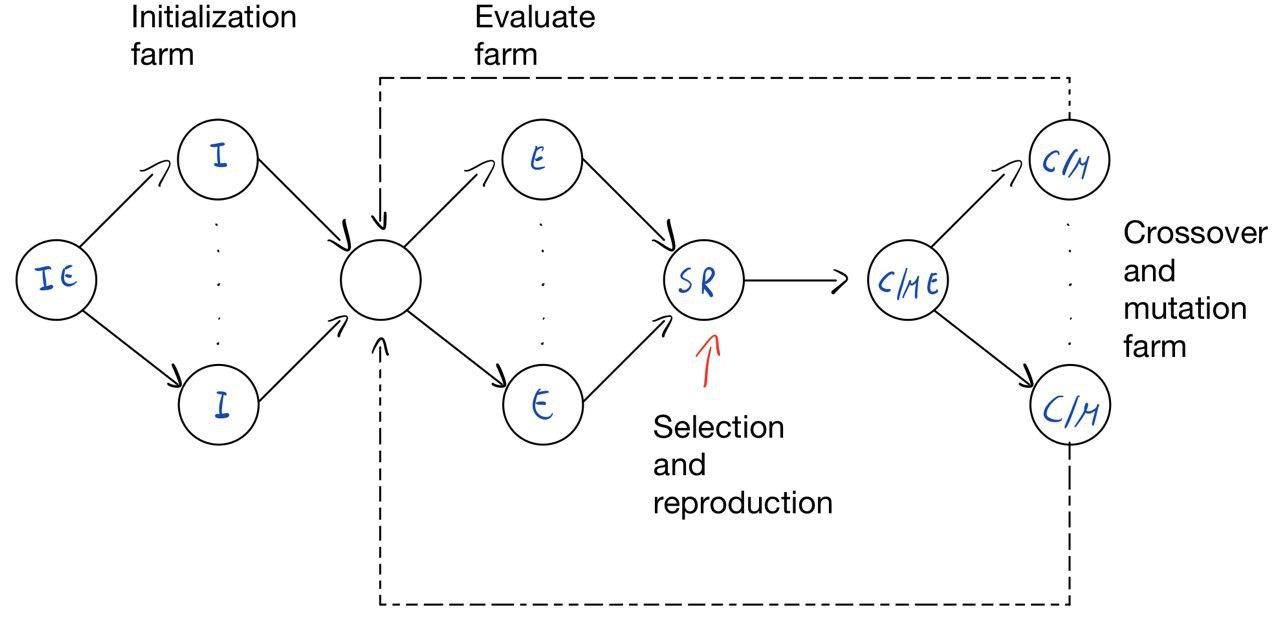
\includegraphics[width=\linewidth]{img/ff_pipeline.jpg}
		\caption{FastFlow pipeline.}
		\label{ff:pipeline}
	\end{figure}
	
	\subsection{Expected performances}
	The developed skeleton is composed of a pipeline $P_{1}$ that has as the first stage the \textit{Initialization} farm $F_{I}$ and as second stage the pipeline $P_{2}$.
	The pipeline $P_{2}$ is composed by two farms, the \textit{Evaluate} farm $F_{E}$ and the \textit{Crossover \& Mutation} farm $F_{CM}$. Each farm has an emitter node and a collector node sometimes shared between farm.
	The service time of the pipeline is the maximum of the service times of the pipeline stages and the service time of a farm is given by the service time of the workers in the farm divided by the number of workers.
	In my implementation, I noticed that the most expensive tasks are the initialization, the evaluation and the crossover of a chromosome. For this reason, the service time strictly depends on the number of chromosome in the population, the number of nodes in the graph and the number of iterations. 

	\section{Results}
	The results are shown in graphs, all the execution are made on Xion Phi machine. The sizes tested are [500, 1000, 2000] chromosomes with a population of size [500, 5000, 2000] with 10 iterations and seed set to 123.
	Some considerations can be done after analysing the plot. First of all, no one of the implementations reaches performances like the ideal. This is due to the overhead inserted by the managing of more threads, in fact we can observe that with more nodes the speedup and scalability rate are slightly better. Moreover, the most interesting thing is that increasing  the population size, the C++ threads implementation have better results than the FastFlow implementation, I think that this is due to the FastFlow implementation of the program in which in the evaluate emitter and the selection reproduction node have to wait for the processing of all chromosomes before they can move on to the next stage. 
	
	\subsection{Speedup curves}
		\subsubsection{With 500 nodes in the graph}
			\begin{figure}[H]
			\centering
			\begin{minipage}[t]{0.32\linewidth}
				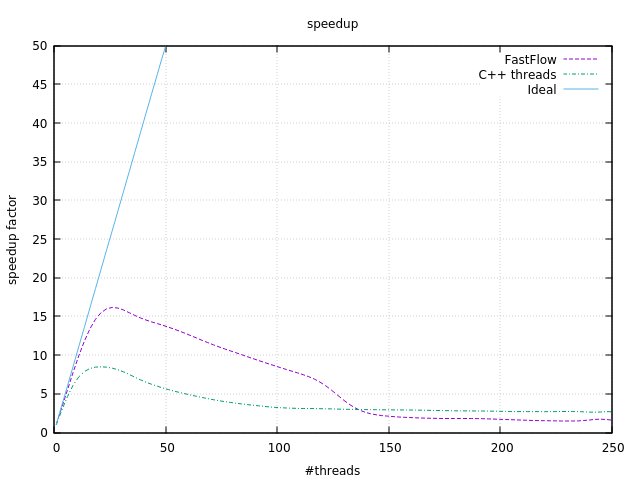
\includegraphics[width=\linewidth]{BenchMarkTSP/speedup/500/SU500500_zoom.png}
				\subcaption{}
			\end{minipage}%
			\begin{minipage}[t]{0.32\linewidth}
				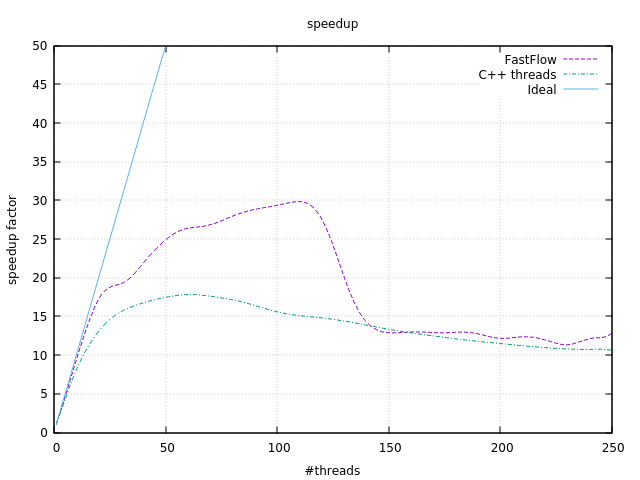
\includegraphics[width=\linewidth]{BenchMarkTSP/speedup/500/SU5005000_zoom.png}
				\subcaption{}
			\end{minipage}
				\begin{minipage}[t]{0.32\linewidth}
				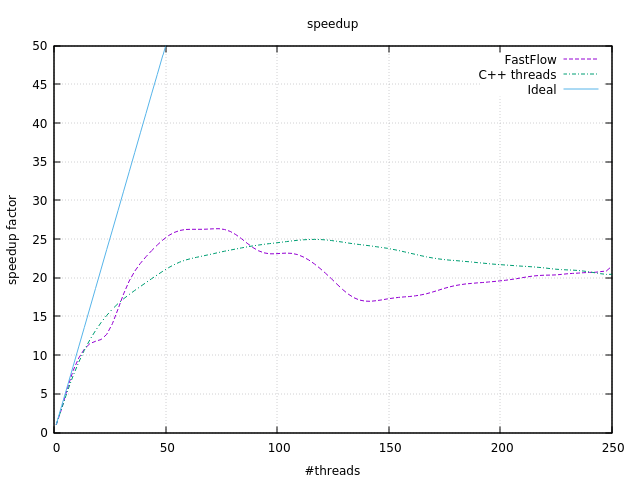
\includegraphics[width=\linewidth]{BenchMarkTSP/speedup/500/SU50020000_zoom.png}
				\subcaption{}
			\end{minipage}
				\caption{Speedup curves for 500 nodes and 500 (a), 5000 (b) and 2000 (c) chromosomes population.}
				\label{500}
			\end{figure}

\begin{center}
	\small\addtolength{\tabcolsep}{5pt}
	\centering
	\begin{longtable}{|c|c|c|c|}
		\hline
		\textbf{Par Deg} & \textbf{\#Population} & \textbf{FastFlow} & \textbf{C++ thread}  \\ \hline
		1        &  500     & 1.034 &  0.968   \\ \hline
		2        &  500     & 2.037 &  1.665   \\ \hline
		32      &  500     & 15.443 &  7.880   \\ \hline
		64      &  500     & 12.197 &  4.516   \\ \hline
		250    &  500     & 1.601 &  2.670   \\ \hline
		1        &  5000   & 1.044 &  0.979   \\ \hline
		2        &  5000   & 2.053 &  1.642   \\ \hline
		32      &  5000   & 18.459 &  16.084   \\ \hline
		64      &  5000   & 25.034 &  18.021   \\ \hline
		250    &  5000   & 12.784 &  10.676   \\ \hline
		1        &  20000 & 0.975 &   1.014  \\ \hline
		2        &  20000 & 2.081 &   1.724  \\ \hline
		32      &  20000 & 19.613 &   18.045  \\ \hline
		64      &  20000 & 24.693 &   21.965  \\ \hline
		250    &  20000 & 21.485 &   20.447  \\ \hline
		\caption{SpeedUp with 500 nodes graph.}	
		\label{tab:dati500}
	\end{longtable}	
\end{center}



		\subsubsection{With 1000 nodes in the graph}
		\begin{figure}[H]
			\centering
			\begin{minipage}[t]{0.32\linewidth}
				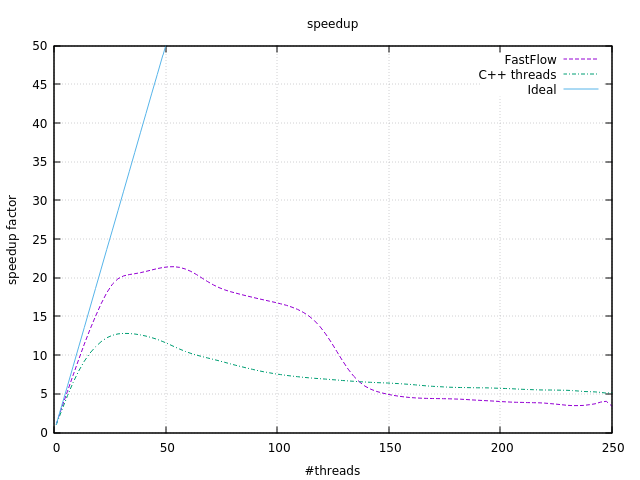
\includegraphics[width=\linewidth]{BenchMarkTSP/speedup/1000/SU1000500_zoom.png}
				\subcaption{}
			\end{minipage}%
			\begin{minipage}[t]{0.32\linewidth}
				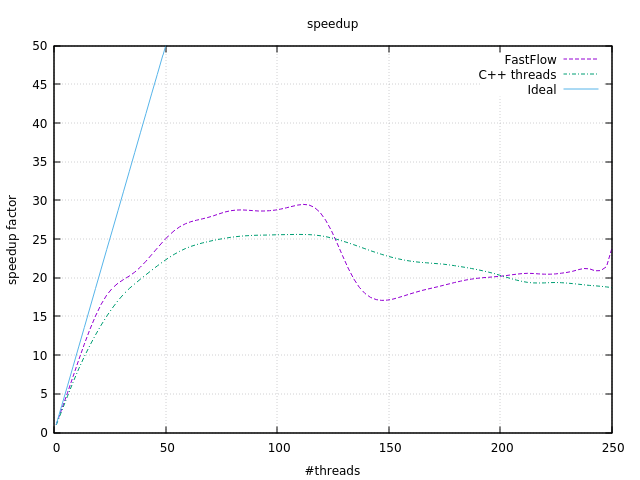
\includegraphics[width=\linewidth]{BenchMarkTSP/speedup/1000/SU10005000_zoom.png}
				\subcaption{}
			\end{minipage}
			\begin{minipage}[t]{0.32\linewidth}
				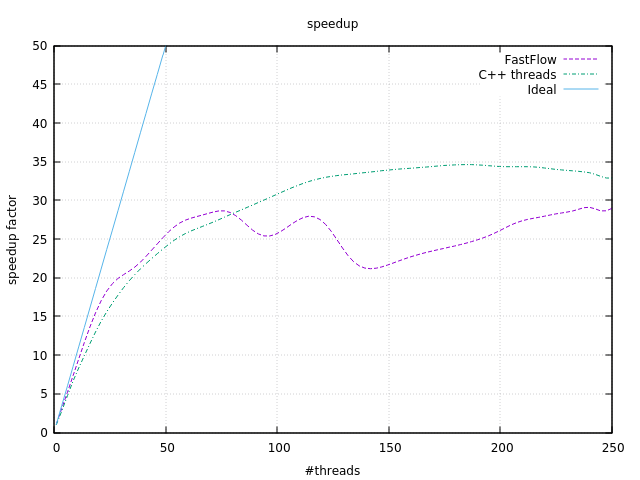
\includegraphics[width=\linewidth]{BenchMarkTSP/speedup/1000/SU100020000_zoom.png}
				\subcaption{}
			\end{minipage}
			\caption{Speedup curves for 1000 nodes and 500 (a), 5000 (b) and 2000 (c) chromosomes population.}
			\label{1000}
		\end{figure}

\begin{center}
	\small\addtolength{\tabcolsep}{5pt}
			\centering
	\begin{longtable}{|c|c|c|c|}
		\hline
		\textbf{Par Deg} & \textbf{\#Population} & \textbf{FastFlow} & \textbf{C++ thread}  \\ \hline
		1         &  500     & 1.049 &  0.984   \\ \hline
		2         &  500     & 2.044 &  1.706   \\ \hline
		32       &  500     & 20.331 &  12.700   \\ \hline
		64       &  500     & 20.078 &  9.736   \\ \hline
		250     &  500     & 3.400 &  5.142   \\ \hline
		1         &  5000   & 1.016 &  0.956   \\ \hline
		2         &  5000   & 1.998 &  1.618   \\ \hline
		32       &  5000   & 18.931 &  18.388   \\ \hline
		64       &  5000   & 26.415 &  23.580   \\ \hline
		250     &  5000   & 23.864 &  18.722   \\ \hline
		1         &  20000 & 1.033 &  0.973   \\ \hline
		2         &  20000 & 2.025 &  1.531   \\ \hline
		32       &  20000 & 19.202 &  19.457   \\ \hline
		64       &  20000 & 26.767 &  26.901   \\ \hline
		250     &  20000 & 28.967 &  32.873   \\ \hline				
		\caption{SpeedUp with 1000 nodes graph.}	
		\label{tab:dati1000}
	\end{longtable}	
\end{center}


		\subsubsection{With 2000 nodes in the graph}
	\begin{figure}[H]
		\centering
		\begin{minipage}[t]{0.32\linewidth}
			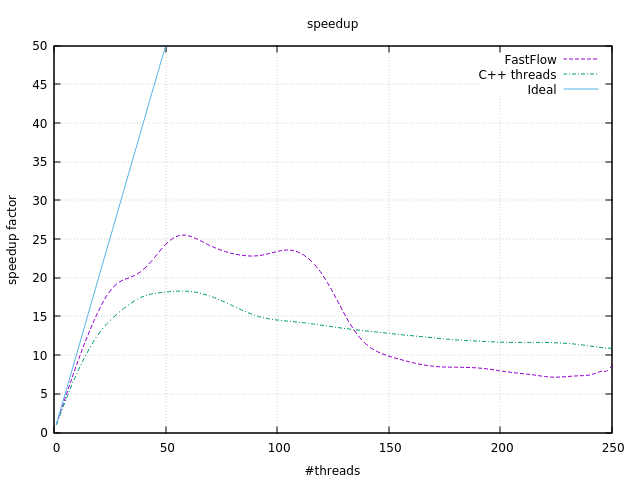
\includegraphics[width=\linewidth]{BenchMarkTSP/speedup/2000/SU2000500_zoom.png}
			\subcaption{}
		\end{minipage}%
		\begin{minipage}[t]{0.32\linewidth}
			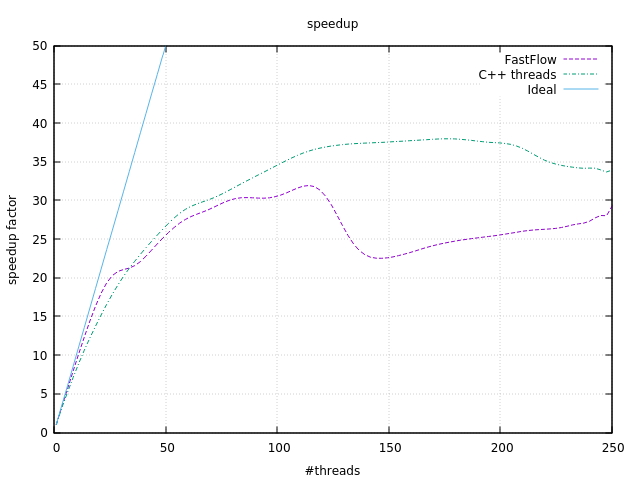
\includegraphics[width=\linewidth]{BenchMarkTSP/speedup/2000/SU20005000_zoom.png}
			\subcaption{}
		\end{minipage}
		\begin{minipage}[t]{0.32\linewidth}
			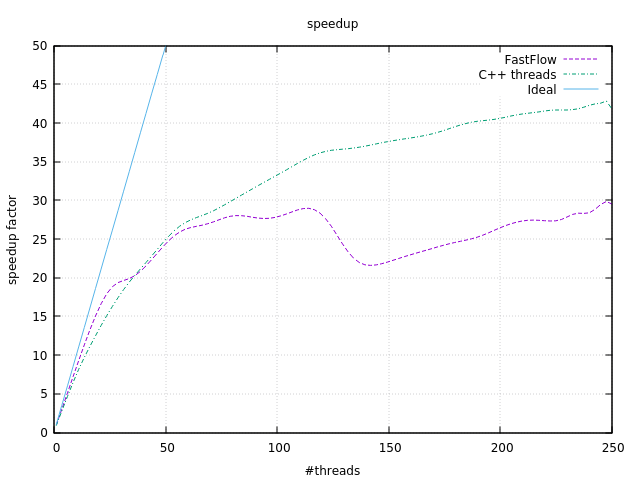
\includegraphics[width=\linewidth]{BenchMarkTSP/speedup/2000/SU200020000_zoom.png}
			\subcaption{}
		\end{minipage}
		\caption{Speedup curves for 2000 nodes and 500 (a), 5000 (b) and 2000 (c) chromosomes population.}
		\label{2000}
	\end{figure}

\begin{center}
	\small\addtolength{\tabcolsep}{5pt}
	\centering
	\begin{longtable}{|c|c|c|c|}
		\hline
		\textbf{Par Deg} & \textbf{\#Population} & \textbf{FastFlow} & \textbf{C++ thread}  \\ \hline
		1         &  500     & 0.959 &  0.902   \\ \hline
		2         &  500     & 1.888 &  1.678   \\ \hline
		32       &  500     & 19.037 &  16.715   \\ \hline
		64       &  500     & 23.163 &  18.406   \\ \hline
		250     &  500     & 8.6560 &  10.898   \\ \hline
		1         &  5000   & 0.990 &  0.952   \\ \hline
		2         &  5000   & 1.990 &  1.939   \\ \hline
		32       &  5000   & 19.881 &  20.847   \\ \hline
		64       &  5000   & 26.952 &  31.090   \\ \hline
		250     &  5000   & 29.290 &  33.899   \\ \hline
		1         &  20000 & 0.906 &  0.876   \\ \hline
		2         &  20000 & 1.809 &  1.598   \\ \hline
		32       &  20000 & 17.992 &  18.861   \\ \hline
		64       &  20000 & 25.130 &  28.805   \\ \hline
		250     &  20000 & 29.526 &  41.830   \\ \hline				
		\caption{SpeedUp with 2000 nodes graph.}	
		\label{tab:dati2000}
	\end{longtable}	
\end{center}

	\subsection{Scalability curves}
		\subsubsection{With 500 nodes in the graph}
		\begin{figure}[H]
			\centering
			\begin{minipage}[t]{0.32\linewidth}
				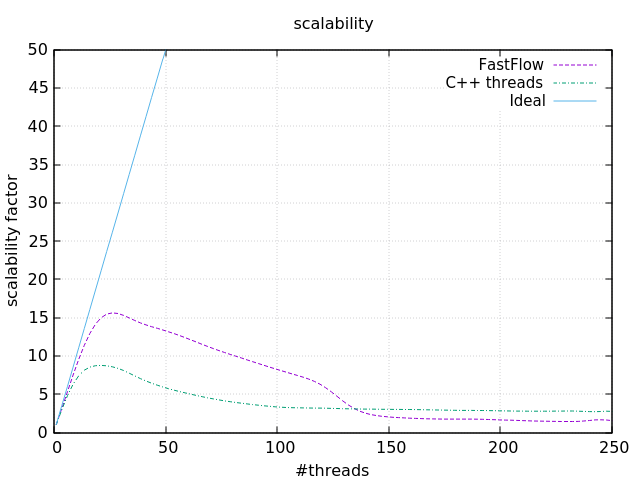
\includegraphics[width=\linewidth]{BenchMarkTSP/scalability/500/SC500500_zoom.png}
				\subcaption{}
			\end{minipage}%
			\begin{minipage}[t]{0.32\linewidth}
				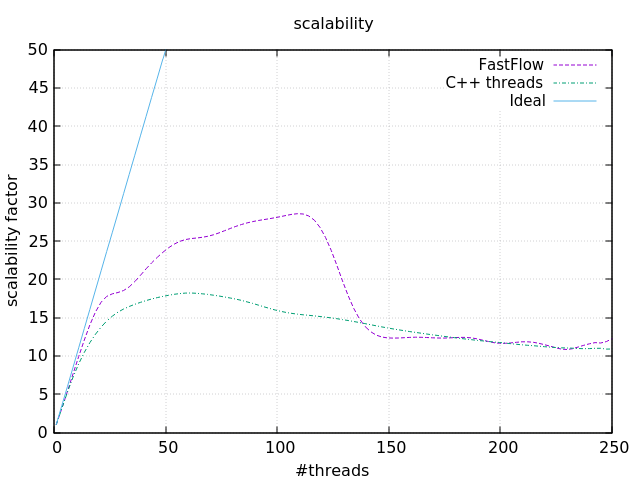
\includegraphics[width=\linewidth]{BenchMarkTSP/scalability/500/SC5005000_zoom.png}
				\subcaption{}
			\end{minipage}
			\begin{minipage}[t]{0.32\linewidth}
				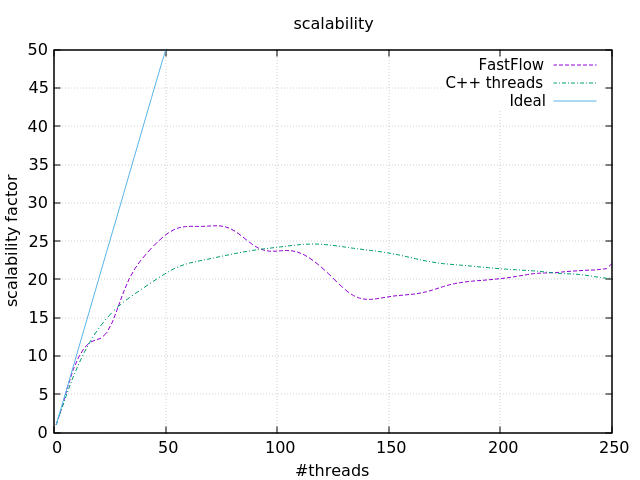
\includegraphics[width=\linewidth]{BenchMarkTSP/scalability/500/SC50020000_zoom.png}
				\subcaption{}
			\end{minipage}
			\caption{Scalability curves for 500 nodes and 500 (a), 5000 (b) and 2000 (c) chromosomes population.}
			\label{500s}
		\end{figure}
	
	\subsubsection{With 1000 nodes in the graph}
		\begin{figure}[H]
			\centering
			\begin{minipage}[t]{0.32\linewidth}
				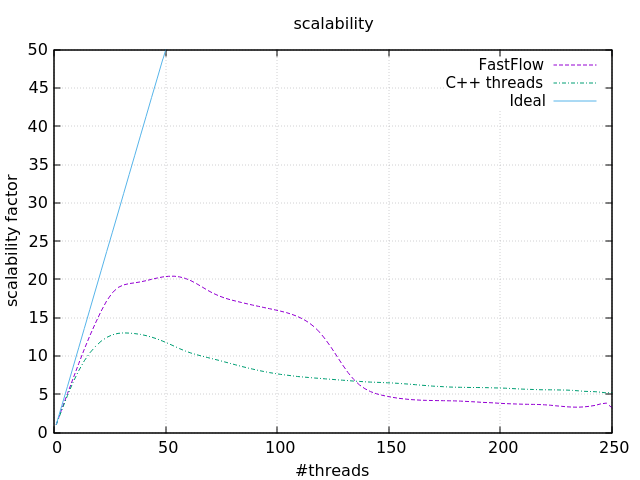
\includegraphics[width=\linewidth]{BenchMarkTSP/scalability/1000/SC1000500_zoom.png}
				\subcaption{}
			\end{minipage}%
			\begin{minipage}[t]{0.32\linewidth}
				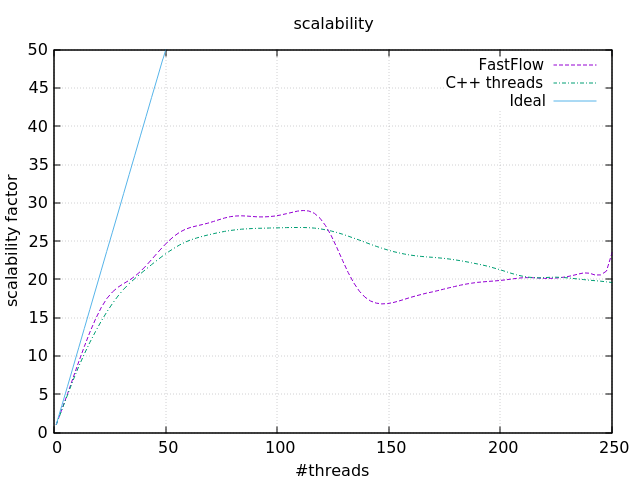
\includegraphics[width=\linewidth]{BenchMarkTSP/scalability/1000/SC10005000_zoom.png}
				\subcaption{}
			\end{minipage}
			\begin{minipage}[t]{0.32\linewidth}
				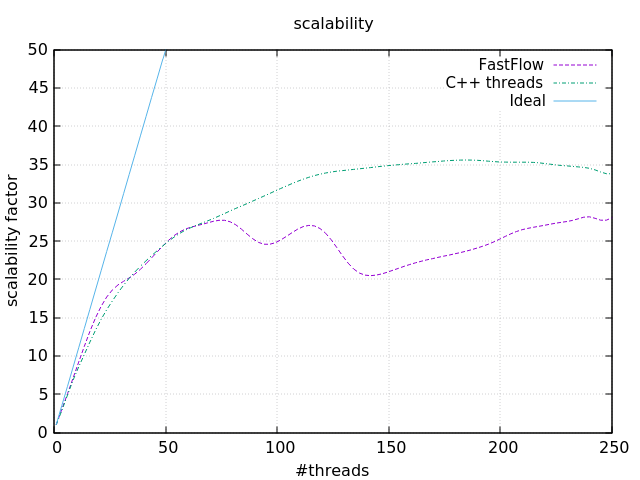
\includegraphics[width=\linewidth]{BenchMarkTSP/scalability/1000/SC100020000_zoom.png}
				\subcaption{}
			\end{minipage}
			\caption{Scalability curves for 1000 nodes and 500 (a), 5000 (b) and 2000 (c) chromosomes population.}
			\label{1000s}
		\end{figure}
	
	\subsubsection{With 2000 nodes in the graph}
		\begin{figure}[H]
			\centering
			\begin{minipage}[t]{0.32\linewidth}
				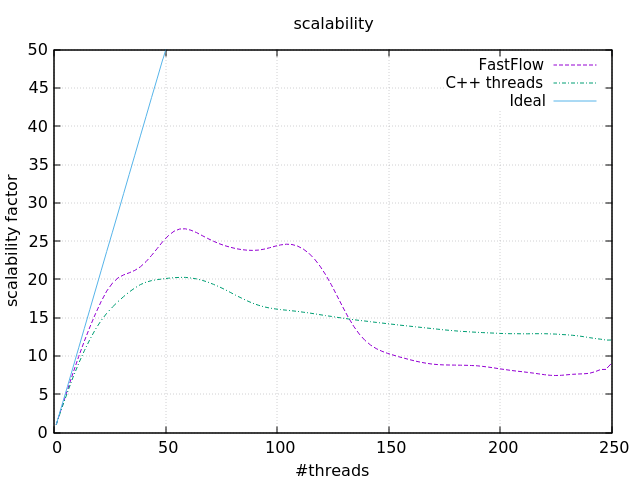
\includegraphics[width=\linewidth]{BenchMarkTSP/scalability/2000/SC2000500_zoom.png}
				\subcaption{}
			\end{minipage}%
			\begin{minipage}[t]{0.32\linewidth}
				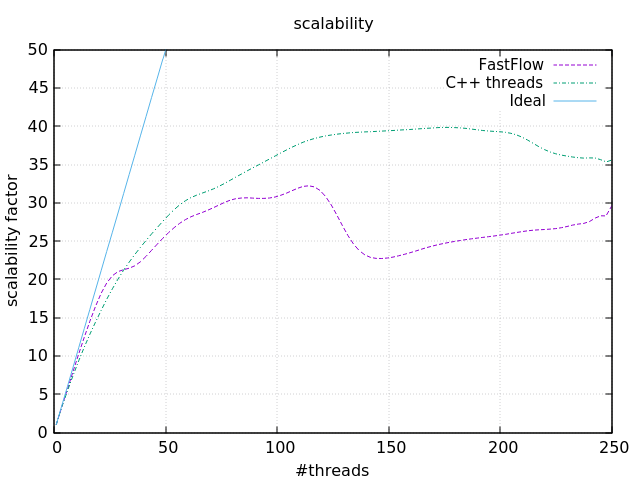
\includegraphics[width=\linewidth]{BenchMarkTSP/scalability/2000/SC20005000_zoom.png}
				\subcaption{}
			\end{minipage}
			\begin{minipage}[t]{0.32\linewidth}
				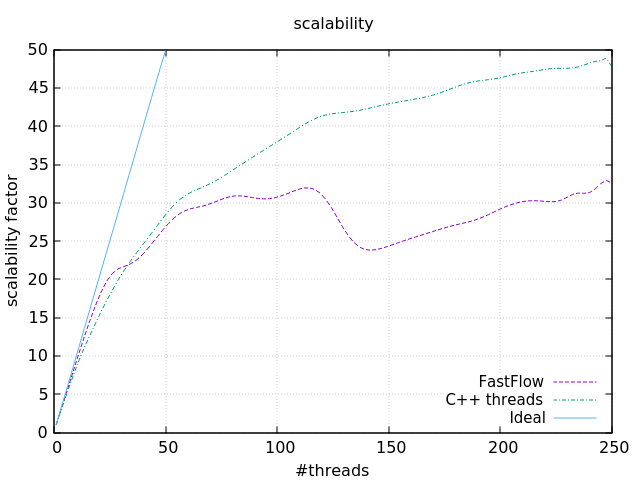
\includegraphics[width=\linewidth]{BenchMarkTSP/scalability/2000/SC200020000_zoom.png}
				\subcaption{}
			\end{minipage}
			\caption{Scalability curves for 2000 nodes and 500 (a), 5000 (b) and 2000 (c) chromosomes population.}
			\label{2000s}
		\end{figure}



\section{Conclusions}
We can see in the graphs that as expected the speedup and the scalability do not increase linearly, but eventually reach an inflexion point and start to decrease or stabilize. This can be attributed to the increasing of the overhead of the splitting. For this reason, it is important to find the right number of parallelism degree and not underestimate the overhead. From the point of view of a programmer, I can say that using a framework is easier than to create the whole parallel application. This because the programmer can focus on the logic and on the parallel skeleton component and not on how to develop the low-level parallel application. 

	\begin{figure}[H]
	\centering
	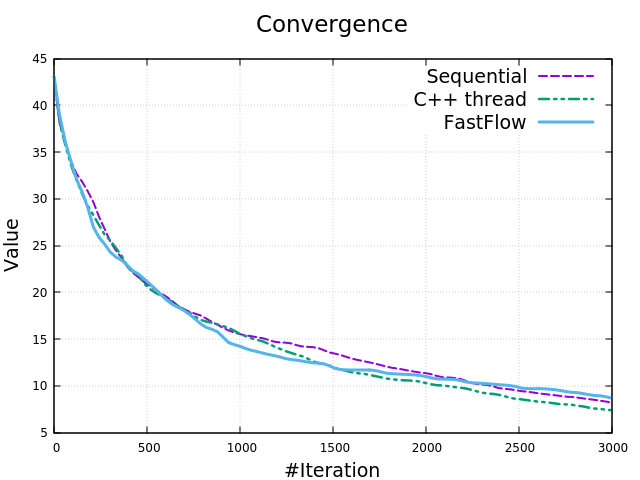
\includegraphics[width=\linewidth]{img/convergence.png}
	\caption{Convergence of the developed algorithms with 200 nodes, 2000 chromosome, 3000 iterations, 1 worker and 1234 as seed.}
	\label{convergence}
\end{figure}


\begin{thebibliography}{9}
	
	\bibitem{GAT} 
	Darrel Whitley.
	\textit{(1994) A Genetic Algorithm Tutorial}. Colorado State University.
	
		
\end{thebibliography}
\end{document}